\documentclass[conference,10pt]{IEEEtran}
\usepackage[T1]{fontenc}
\usepackage{amsmath,amssymb}
\usepackage{graphicx}
\usepackage{booktabs}
\usepackage{url}
\usepackage[hidelinks]{hyperref}
\usepackage[font=footnotesize]{caption}
\graphicspath{{../results/figures/}}

% Slightly tighter spacing so the content fits in two pages.
\setlength{\textfloatsep}{6pt plus 2pt minus 2pt}
\setlength{\floatsep}{5pt plus 2pt minus 2pt}
\setlength{\abovedisplayskip}{3pt}
\setlength{\belowdisplayskip}{3pt}

\begin{document}

\title{MergeRL: Learning Safe Highway\\On-Ramp Merging with PPO}

\author{\IEEEauthorblockN{Hitesh Saini (B24CM1029)}
\IEEEauthorblockA{IIT Jodhpur, AI Course -- Assignment 2 (RL Mini Project)\\
GitHub: \url{https://github.com/hitesh771/mergerl}}}

\maketitle

\begin{abstract}
On-ramp merging is a frequent cause of hard braking and rear-end collisions.
We formulate it as a Markov Decision Process in which an ego car on an
acceleration lane controls its longitudinal acceleration and must merge into
dense highway traffic driven by the Intelligent Driver Model (IDM). We
implement the simulator, PPO and Double DQN from scratch, and compare them with
rule-based gap-acceptance and IDM baselines. Across 3 seeds and
3{,}600 evaluation episodes per agent, PPO merges in 99.4\% of episodes with
1 collision in 2{,}400 on the training densities, and keeps 70.5\% success on unseen
heavier traffic where the best rule-based baseline drops to 11.2\%.
\end{abstract}

\section{Problem and Environment}
A single-lane highway (0--700\,m) is joined by an acceleration lane whose merge
zone spans 200--320\,m and ends in a hard barrier. The simulator is a 1-D
longitudinal point-mass model written in NumPy ($\Delta t=0.1$\,s; the agent
acts every 2 sub-steps, i.e.\ 5\,Hz). Highway cars follow the IDM,
\begin{equation*}
a = a_{\max}\Big[1-\big(\tfrac{v}{v_0}\big)^4-\big(\tfrac{s^*}{s}\big)^2\Big],\quad
s^* = s_0+vT+\tfrac{v\,\Delta v}{2\sqrt{a_{\max} b}},
\end{equation*}
with the constant-acceleration heuristic for cut-ins and braking capped at
8\,m/s$^2$. Every car samples its driver type between \emph{cautious}
($v_0{=}24$\,m/s, $T{=}1.8$\,s) and \emph{aggressive} ($v_0{=}33$\,m/s,
$T{=}1.0$\,s); the density $\rho$ is sampled per episode and inflow is
steady. The ego changes lane automatically once it is inside the zone and both
bumper gaps exceed only 2\,m. Unsafe cut-ins are therefore \emph{possible}: the
lag car may brake hard or crash, so the agent has to learn \emph{when and at
what speed} to arrive next to a good gap. An episode ends in a collision,
at the ramp end, after 40\,s, or 8\,s after a merge (success). The env
follows the Gymnasium API and is fully seeded.

\begin{figure*}[t]
\centering
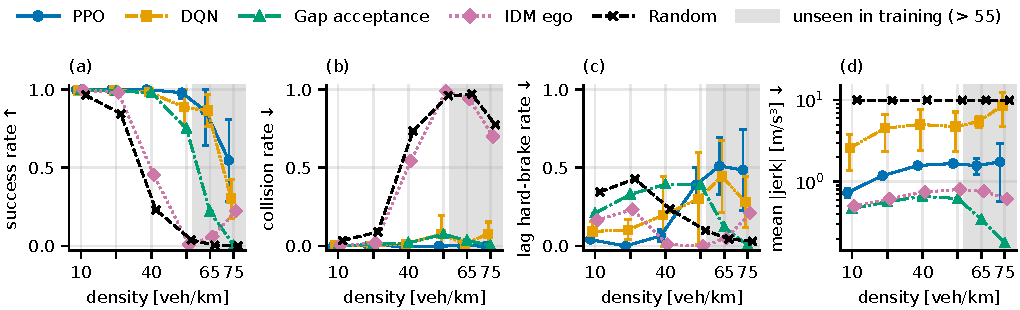
\includegraphics[width=\textwidth]{density_sweep.pdf}
\caption{Density sweep over 200 episodes per density (mean $\pm$1 std over 3
seeds for PPO/DQN). The shaded region was never seen in training. PPO
keeps success near 1 with almost no collisions and keeps the highest success
in unseen traffic, at the cost of more lag-car hard braking there.}
\label{fig:sweep}
\end{figure*}

\section{RL Formulation}
\textbf{State $\mathcal{S}\subset\mathbb{R}^{13}$} (continuous, scaled to
$\approx[-1,1]$): ego speed; ego position relative to the zone; distance to the
ramp end; merged flag; gap and relative speed to the highway \emph{lead} and
\emph{lag} cars; lag-car time-to-collision (TTC, clipped to 10\,s); lag-car
speed; lag-car time headway; traffic density; previous acceleration (so the
policy can see the jerk it causes). Gaps are relative to the ego's
longitudinal position, so a negative gap means a car is alongside.

\textbf{Action $\mathcal{A}=[-1,1]$} (continuous), scaled to an acceleration in
$[-3,3]$\,m/s$^2$. For DQN it is discretised into 7 levels
$\{-3,-2,\dots,3\}$\,m/s$^2$.

\textbf{Reward $\mathcal{R}$} per decision step:
\begin{equation*}
\begin{split}
r_t ={}& 0.05\,\tfrac{v}{v_{\max}} - 0.02\,\tfrac{|a_t-a_{t-1}|}{6}
- 0.3\,\mathbf{1}[\text{TTC}<2\text{\,s}] \\
&- 2.0\,\mathbf{1}[a_{\text{lag}}<-4] - 0.1\,\mathbf{1}[\neg\text{merged}\wedge v<2] - 0.02
\end{split}
\end{equation*}
plus events: $+5$ on merging, $+5$ for surviving 8\,s after it, $-20$ for a
collision, $-10$ for reaching the ramp end unmerged. The terms reward
progress, comfort, safe spacing and courtesy (not forcing the car behind to
brake harder than 4\,m/s$^2$). The standstill penalty stops the reward hack of
waiting on the ramp forever, and failing costs less than crashing.

\section{Algorithms and Baselines}
\textbf{PPO} (own PyTorch implementation): Gaussian actor and value critic
(2$\times$64 tanh MLPs, state-independent $\log\sigma$), 16 parallel envs
$\times$ 256 steps per update, GAE ($\gamma{=}0.99$, $\lambda{=}0.95$), clipped
surrogate ($\epsilon{=}0.2$), 10 epochs $\times$ 8 minibatches, advantage and
running observation normalisation, gradient clipping 0.5, and linearly decaying
learning rate $3{\times}10^{-4}$. We use a \textbf{density curriculum}:
10--20\,veh/km for the first 20\% of training, then 10--40, then 10--55. We
train for 3M steps with 3 seeds.
\textbf{Double DQN} (own): 2$\times$128 ReLU Q-network, replay 200k, Huber
loss, hard target update every 2k steps, $\epsilon$ decayed from 1 to 0.05
over 30\%; we train for 1M steps with 3 seeds ($\sim$5$\times$ slower).
\textbf{Baselines} (comparison only): (i) \emph{Gap acceptance}, which plans a
constant acceleration so that the ego arrives at the zone together with the
gap ($\geq$10\,m) whose speed best matches its own, then follows with IDM;
(ii) \emph{IDM ego}, which follows the ramp leader and merges as soon as it is
allowed; (iii) \emph{Random}.
Evaluation uses scenario seeds ($\geq$1000) disjoint from training, 200
episodes at each density $\rho\in\{10,25,40,55\}$ (seen) and $\{65,75\}$
(\emph{unseen}).

\begin{figure}[t]
\centering
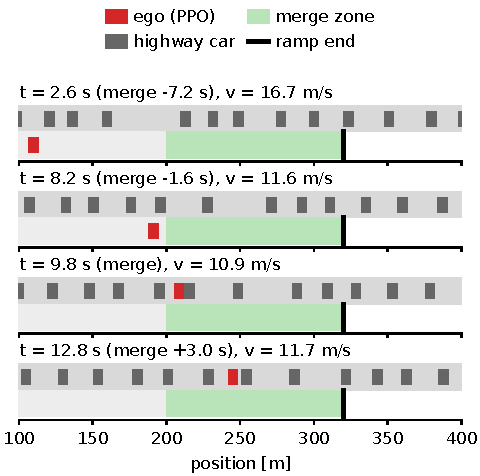
\includegraphics[width=0.85\columnwidth]{merge_snapshot.pdf}
\caption{A PPO episode at 40\,veh/km: the agent slows down on the ramp to line
up with a gap, merges at 9.8\,s and then follows the traffic.}
\label{fig:snap}
\end{figure}

\section{Results}
\begin{figure}[t]
\centering
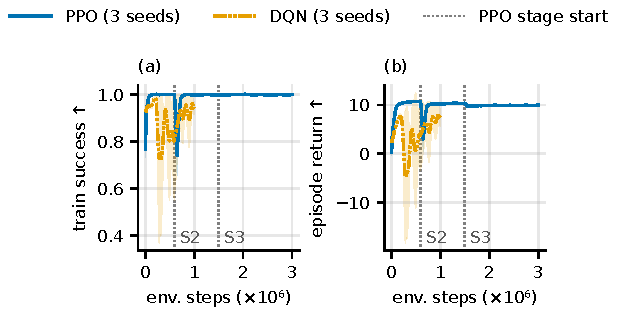
\includegraphics[width=\columnwidth]{learning_curves.pdf}\\[2pt]
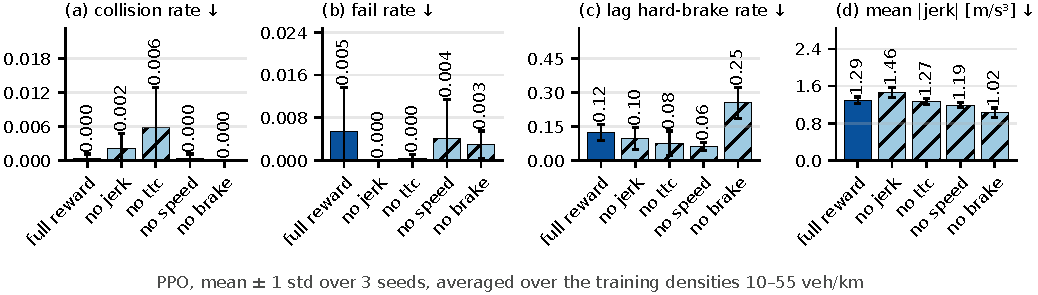
\includegraphics[width=\columnwidth]{ablation.pdf}
\caption{(a,b) training curves (mean $\pm$1 std over 3 seeds, 50k-step rolling
mean; S2/S3 = curriculum stages). (c,d) reward ablation, PPO retrained
with one term removed (3 seeds, $\rho\le55$).}
\label{fig:lc}
\end{figure}

\begin{table}[t]
\centering
\caption{Mean over seeds and densities (200 episodes/density). HB = share of
episodes where the lag car brakes harder than 4\,m/s$^2$.}
\label{tab:main}
\setlength{\tabcolsep}{3.2pt}
\footnotesize
\begin{tabular}{@{}lcccccc@{}}
\toprule
 & \multicolumn{4}{c}{Seen ($\rho\le55$)} & \multicolumn{2}{c}{Unseen (65, 75)}\\
\cmidrule(lr){2-5}\cmidrule(l){6-7}
Agent & Succ.$\uparrow$ & Coll.$\downarrow$ & HB$\downarrow$ & |jerk|$\downarrow$ & Succ.$\uparrow$ & Coll.$\downarrow$\\
\midrule
\textbf{PPO}   & \textbf{0.994} & \textbf{0.0004} & 0.13 & 1.29 & \textbf{0.705} & \textbf{0.001}\\
DQN            & 0.965 & 0.025 & 0.17 & 4.22 & 0.584 & 0.046\\
Gap accept.    & 0.930 & 0.026 & 0.33 & \textbf{0.58} & 0.112 & 0.020\\
IDM ego        & 0.610 & 0.390 & \textbf{0.10} & 0.67 & 0.143 & 0.820\\
Random         & 0.520 & 0.455 & 0.28 & 9.99 & 0.002 & 0.872\\
\bottomrule
\end{tabular}
\end{table}

\textbf{Learning.} PPO reaches $\approx$100\% training success within 0.1M
steps; the dip at the start of each curriculum stage recovers within $\sim$0.15M
steps (Fig.~\ref{fig:lc}a,b). DQN learns too, but it is less stable across seeds
and stage changes.

\textbf{Comparison} (Table~\ref{tab:main}, Fig.~\ref{fig:sweep}). On the
training densities PPO has 1 collision in 2{,}400 episodes (DQN: 60) and
forces the lag car to brake hard $2.6\times$ less often than gap acceptance,
while it merges faster (7.8 vs.\ 9.8\,s) and drives faster (17.5 vs.\
14.4\,m/s). At 55\,veh/km gap acceptance succeeds in only 75\% of episodes,
against 98\% for PPO. IDM ego is fast but crashes in dense traffic, because a
greedy merge rule ignores the lag car. On unseen 65--75\,veh/km traffic PPO
degrades gracefully (70.5\% success, 0.1\% collisions) and fails safely at the
ramp end instead of crashing, though it forces more hard braking (HB 0.50). Gap acceptance collapses there (11.2\%), because
gaps of 10\,m or more stop appearing. DQN's 7 coarse actions cause
3$\times$ PPO's jerk, which favours a continuous policy.

\textbf{Reward ablation} (Fig.~\ref{fig:lc}c,d). Each term does what it was
designed for. Without the brake term the lag-car hard-brake rate doubles
(0.12$\to$0.25), because the agent cuts in more aggressively. Without the
jerk term $|$jerk$|$ rises (1.29$\to$1.46). Removing the TTC term gives the
highest collision rate. Without the speed term the agent is 22\% slower (17.5$\to$13.6\,m/s).

\textbf{Limitations.} PPO is still about 2$\times$ jerkier than the smooth
rule-based planner. Raising the jerk weight to 0.1--0.5 did \emph{not} reduce
jerk, but did raise lag-car hard braking up to 4$\times$ in unseen traffic, so
we kept 0.02. Action filtering, multi-lane traffic and learning highway
drivers (multi-agent RL) are future work.

\textbf{Reproducibility.} \texttt{bash scripts/run\_all.sh} runs the tests,
then trains (seeds 0--2), evaluates and plots everything ($\sim$2.5\,h on 12
CPU cores). The trained checkpoints are in \texttt{checkpoints/}.


\begin{thebibliography}{9}\footnotesize
\bibitem{ppo} J.~Schulman \emph{et al.}, ``Proximal policy optimization algorithms,'' arXiv:1707.06347, 2017.
\bibitem{gae} J.~Schulman \emph{et al.}, ``High-dimensional continuous control using generalized advantage estimation,'' ICLR, 2016.
\bibitem{ddqn} H.~van Hasselt, A.~Guez, D.~Silver, ``Deep reinforcement learning with double Q-learning,'' AAAI, 2016.
\bibitem{idm} M.~Treiber, A.~Hennecke, D.~Helbing, ``Congested traffic states in empirical observations and microscopic simulations,'' Phys.\ Rev.\ E, 62(2), 2000.
\bibitem{cah} A.~Kesting, M.~Treiber, D.~Helbing, ``Enhanced intelligent driver model to access the impact of driving strategies on traffic capacity,'' Phil.\ Trans.\ R.\ Soc.\ A, 368, 2010.
\end{thebibliography}

\end{document}
